%!TEX root = ../../report.tex
\section{Learning Markov Parameters for Dynamic Obstacles}
\label{sec:learning_markov_evaluation}
The PMAC methods ability to learn the Markov parameters; $\lambda_{entry}$ and $\lambda_{exit}$, is evaluated by navigating a MiR-100 robot along the path shown in figure \ref{fig:flexlab_path_with_covariance_with_cleaned_map} for an hour while learning the parameters with the method.

\begin{figure}[htbp]
    \begin{subfigure}[t]{0.7\textwidth}	
        \centering	
        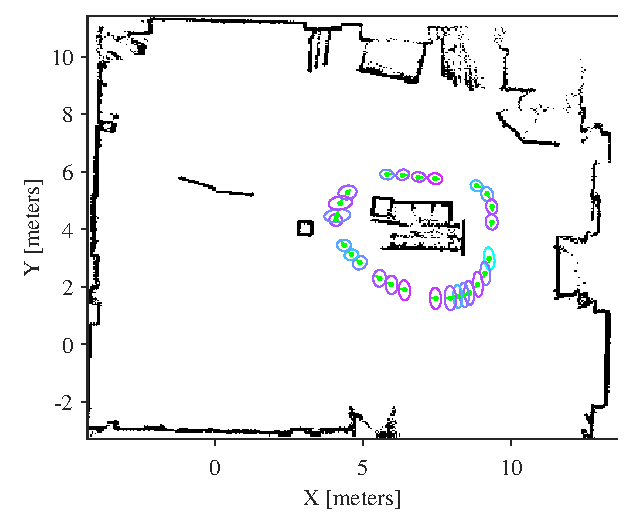
\includegraphics[scale=1.0]{chapters/evaluation/figures/flexlab_path_with_covariance_with_cleaned_map}
    \end{subfigure}
    \begin{subfigure}[t]{0.2\textwidth}
        \centering
        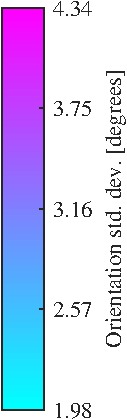
\includegraphics[scale=1.0]{chapters/evaluation/figures/flexlab_path_with_covariance_bar-crop}
    \end{subfigure}
    \caption{Covariances estimated by AMCL, superimposed on the used static map, shown with contours marking one standard deviation around the robot's estimated pose(green).}
    \label{fig:flexlab_path_with_covariance_with_cleaned_map}
\end{figure}

Once every minute the boxes shown in figure \ref{fig:cells_used_for_evaluation_with_identification} are moved from  the initial pose(Blue) to the alternative one(Red). 
The boxes are however only moved if a random number between one and zero is above the probability for the box changing state from it current state.
The probability for a box moving away from its initial pose is hence given by $\lambda_{exit}$ and the probability for it moving back to its initial pose is given by $\lambda_{entry}$.
These values are shown in yellow in figure \ref{fig:compare_learned_markov_entry} and \ref{fig:compare_learned_markov_exit} compared with the median of the learned ones for each box.
The median estimate of the cells indicated in figure \ref{fig:cells_used_for_evaluation_with_identification} for each box pose is used to avoid having influence from the cells with wrongly estimated parameters since they are only rarely observed.

\begin{figure}
    \centering
    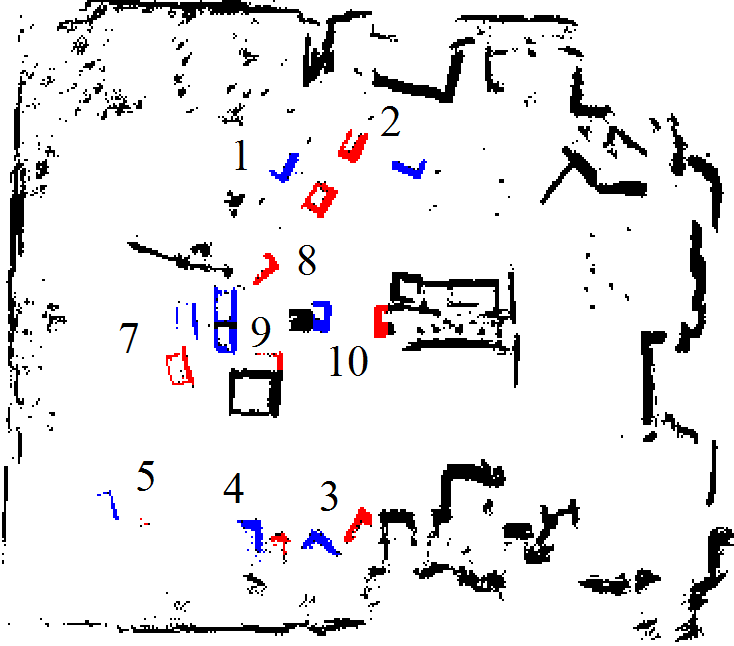
\includegraphics[scale=1.0]{chapters/evaluation/figures/cells_used_for_evaluation_with_identification}
    \caption{Map of PMAC cells with an occupied count value larger than $0.5$, where the cells used for evaluation is indicated at their initial(blue) and alternative(red) positions.}
    \label{fig:cells_used_for_evaluation_with_identification}
\end{figure}

The PMAC is updated with probabilities from the static map once every minute, so the parameters for the cells are estimated using only around $60$ updates for the cells at the boxes poses for the boxes that are always visible to the robot when it moves past them.
This is for example not the case for box number one and six, so they are observed fewer times.

\subsection{Results}
By comparing the learned $\lambda_{entry}$ with the actual once in figure \ref{fig:compare_learned_markov_entry} it is clear that the estimations are generally too low except for all the boxes except number five.
For unknown reasons the entry event counter follows the free counter for this cell, which results in a $\lambda_{entry}$ close to one when applying equation \vref{eq:pmac_lambda}.

\begin{figure}
    \centering
    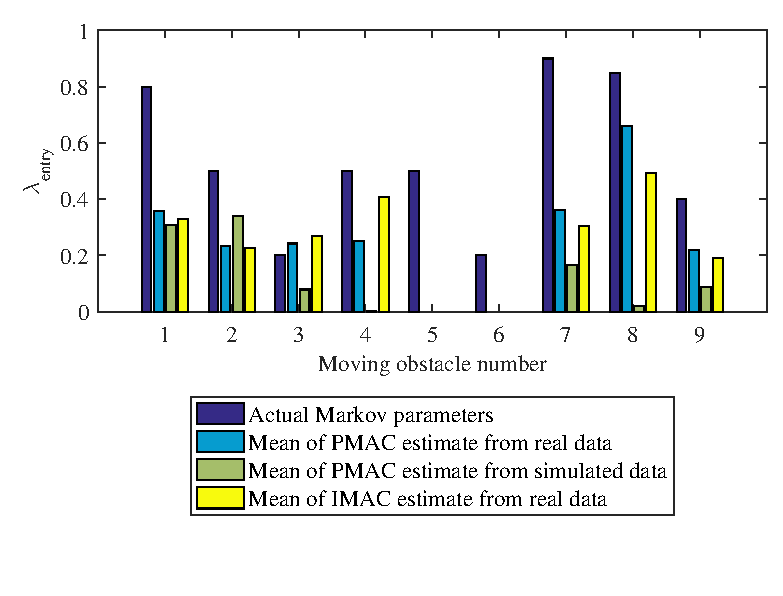
\includegraphics[scale=1]{chapters/evaluation/figures/compare_learned_markov_entry}
    \caption{Comparison of the median estimated $\lambda_{entry}$ with the ones governing the Markov process for the boxes.}
    \label{fig:compare_learned_markov_entry}
\end{figure}

The estimated $\lambda_{exit}$ values are much closer to the actual  parameters of the Markov processes governing the movements of the obstacles.
The median $\lambda_{exit}$ for box number five is zero since none exit events was observed since it was too far away to be inserted with the used reduced ideal sensor model described in section \vref{sec:reduced_ideal_sensor_model}.
The estimated $\lambda_{exit}$ is quite wrong for box number six since it is often not observed when box seven and eight are at their initial pose.

\begin{figure}
    \centering
    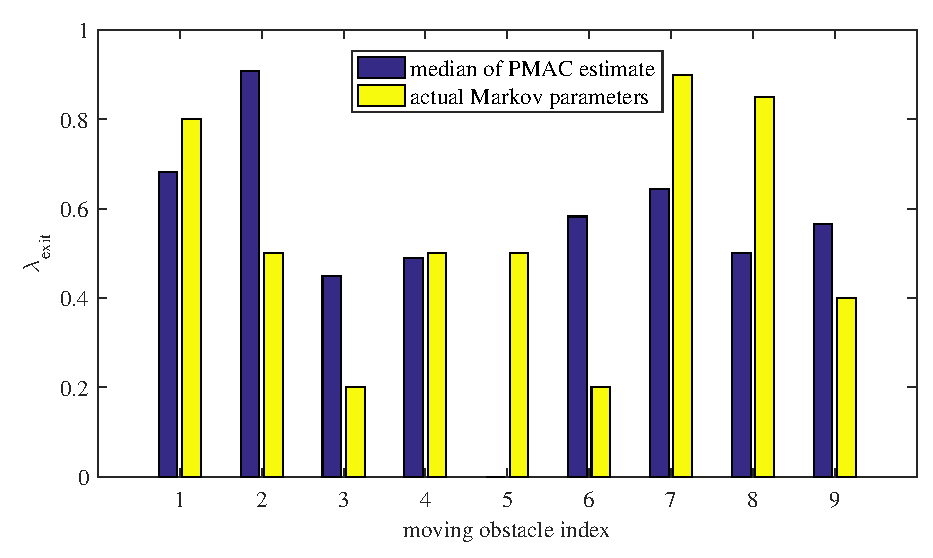
\includegraphics[scale=1]{chapters/evaluation/figures/compare_learned_markov_exit}
    \caption{Comparison of the median estimated $\lambda_{exit}$ with the ones governing the Markov process for the boxes.}
    \label{fig:compare_learned_markov_exit}
\end{figure}

\subsection{Ability to Learn Dynamics of environment}
The proposed PMAC methods ability to learn the dynamic behavior was investigated by letting it learn from observations of obstacles moving with a controlled Markov process.
The errors in the estimated Markov parameters when using the PMAC learner described in section \ref{sec:learning_markov_evaluation} most likely stems from unmodeled localization errors and insufficient number of observations. 

The wrong estimates for lambda $\lambda_{entry}$ might be due to the fact that cells near the edges of obstacles are often wrongly observed free when the end of the ray-traced lines are too long due to errors in the estimated robot pose.
When the lines are too short due to localization errors the cells further from the laser in the direction of the line are however not counted up as occupied.
This causes an increase in free count values compared to the ones in the entry event counter, which results in the $\lambda_{entry}$ values being too small.
The estimated $\lambda_{exit}$ do not suffers from this problem and are also better, but the small amount of measurements is simply not sufficient to achieve accurate estimates for all the boxes.

Despite the fact that it cannot be shown that PMAC learns the dynamics of semi-static obstacles fast,
the method is useful to improve prediction of future probability for occupied and location of static obstacles.